% ...

%%%%%%%%%%%%%%%%%%%%%%%%%%%%%%%%%%%%%%%%%%%%%%%%%%%%%%%%%%%%%%%%%%%%%

\documentclass[11pt, a4paper, titlepage]{article}
\usepackage[left=2cm, right=2cm, text={19cm, 25cm},
            top=3cm, bottom=3cm]{geometry}
\usepackage[utf8]{inputenc}
\usepackage[czech]{babel}
\usepackage{pdfpages}
\usepackage[obeyspaces]{url}
% \usepackage{framed}
% \usepackage[T1]{fontenc}
% \usepackage{lmodern}
\usepackage{enumitem}
\usepackage{graphicx}
\usepackage{float}

\usepackage{caption}
\usepackage{subcaption}



\setlength\parindent{0pt}

%%%%%%%%%%%%%%%%%%%%%%%%%%%%%%%%%%%%%%%%%%%%%%%%%%%%%%%%%%%%%%%%%%%%%

\begin{document}

\begin{titlepage}
    \begin{center}
        \begin{figure}[htb]
            \centering
            
\includegraphics[width=0.85\hsize]{images/fitlogo.pdf}
        \end{figure}

        \vspace{\stretch{0.382}}

        {\LARGE Tvorba uživatelského rozhraní} \\
        \bigskip
        \smallskip
        {\Huge Technická zpráva} \\
        \bigskip
        \smallskip
        {\LARGE Informační systém pro florbalovou ligu}
        \vspace{\stretch{0.618}}

    \end{center}
    % {\Large \today \hfill Vladimír Dušek, xdusek27}
    Číslo projektu: 100, Vlastní zadání \\
    Číslo a název týmu: 25, Tým xdusek27 \\
    Autor: Vladimír Dušek (xdusek27) \\
    Další členové týmu: nejsou \\
\end{titlepage}

%%%%%%%%%%%%%%%%%%%%%%%%%%%%%%%%%%%%%%%%%%%%%%%%%%%%%%%%%%%%%%%%%%%%%

\tableofcontents

\newpage

%%%%%%%%%%%%%%%%%%%%%%%%%%%%%%%%%%%%%%%%%%%%%%%%%%%%%%%%%%%%%%%%%%%%%

\section{Abstrakt}

Informační systém bude sloužit primárně hráčům a fanouškům Orlické amatérské florbalové ligy (OAFL). Avšak může posloužit i jiným florbalovým ligám, či ligám ve sportovním systému florbalu podobném. OAFL se hraje již od roku 2010 a zájem o~ní stoupá. Organizátoři jsou primárně nadšenci pro florbal, soutěž organizují pro radost ze sportu, disponují minimálním ziskem. Doposud se výsledky, statistiky, rozpisy a veškeré informace zveřejňovali pouze na facebookové stránce OALF. Informační systém by tedy zpřehlednil veškeré informace, dal jim jasný řád a navíc i přehledně archivoval výsledky z~uplynulých ročníků. Zároveň by nabízel informace nové. Například statistiky za celou sezónu, kolik padlo gólů, kolik bylo uděleno trestných minut a podobně. Informační systém by samozřejmě ulehčil práci organizátorům, respektive zkrátil potřebný čás pro správu všech informací. Administrátor soutěže by měl k~dispozici rozhraní pomocí kterého by mohl vkládat rozpis zápasů a poté jejich výsledky. Veškeré informace by se promítli a aktualizovali na mnoha místech automaticky.

%%%%%%%%%%%%%%%%%%%%%%%%%%%%%%%%%%%%%%%%%%%%%%%%%%%%%%%%%%%%%%%%%%%%%

\section{Průzkum kontextu použití}

\subsection{Cílová skupina}

Cílová skupina jsou hráči a fanoušci OAFL, florbalový nadšenci. Převažují muži nejčastěji ve věku od 15 do 35 let. Jedná se o~studenty případně pracující lidi. Jejich znalosti práce s výpočetní technikou jsou průměrné, nejčastěji se jedná o~běžné uživatele internetu a sociálních sití. V~případě fanoušků může být skupina mírně rozsáhlejší, většinou se jedná o~rodinné příslušníky hráčů.

\subsection{Persóna}

Jiřímu je 20 let. Studuje Vysokou Školu Ekonomickou v~Praze. Má rád sport, ale nechce se jim živit. Je to pro něho koníček, ale zároveň má rád soutěživost. Je obecně pohybově nadaný a vyzkoušel si velké množství sportů. OAFL je pro něho zpestření víkendu od učení a brigád. Také se zde rád vidí s~kamarády ze střední školy, se kterými udržuje vztahy.

\begin{figure}[H]
    \centering
    
\includegraphics[width=.70\textwidth]{images/persona.jpg}\hfill
    \caption{Typický uživatel}
    \label{fig:persona}
\end{figure}


\subsection{Typické případy použití}

\begin{itemize}
    \item Hráč se podívá kdy hraje zápasy.
    \item Hráč zjistí jak si vede jeho tým v~tabulce, případně on sám.
    \item Tým analyzuje svoje šance postupu do play-off a sleduje jak se daří jeho rivalům.
    \item Fanoušek objeví atraktivní utkání, která by stálo za to vidět.
    \item Fanoušek najde jak si vede jeho oblíbený tým.
    \item Florbalový nadšenec, zatím ne hráč OAFL, najde kde se liga hraje, jakým systémem se hraje, kolik je startovné a jak se může přihlásit.
    \item Rodinný příslušník hráče má přehled o~tom, kdy hráč hraje zápasy a nemůže se učástnit žádných jiných aktivit.
\end{itemize}

\subsection{Prostředí použití}

V~práci, ve škole, ve volném čase, v~podstatě kdykoliv kdy si hráč bude potřebovat zjistit například kdy hraje a tomu přizpůsobit svůj program. Web by měl tedy dobře vypadat jak na počítači tak na mobilním zařízení.
\bigskip

Konkrétní situace, hráč sedí v~páteční podvečer v~restauračním zařízení a je velmi spokojen, rozhodně neplánuje odejít brzy. Potřebuje tedy nutně zjistit v~kolik hodin následujicí den hraje, aby si mohl nastavit budík. V~opačném případě by hrozilo, že by nemusel zavčas procitnout.
\bigskip

Další situace, hráčova partnerka plánuje svého muže mile překvapit něčím, o~co velmi stojí, například romantickým víkendem v~Benátkách. Může si tak na webu OAFL najít, které víkendy má muž již zabrané a vyhnout se tak případným, nepříjemným konfliktům.

\subsection{Požadavky na produkt}

V~současné době hledání veškerých informací na facebookové stránce není ani trochu praktické. Je nepřehledné, všechny informace jsou na jednom místě -- zdi. Zejména složité je pak dohledávání starších příspěvků. Například výsledky několik kol dozadu. Nedejbože pak statistiky z~loňských sezón.
\bigskip

Logika aplikace bude spoustu věcí sama vypočítávat a při zadání pouze výsledku zápasu, střelců gólů a dalších nezbytných informací vše sama aktualizuje. Uživateli se poté vše zobrazí v~přehledných tabulkách a rozpisech. Mezi nimi bude překlikávat v~intuitivním menu.

%%%%%%%%%%%%%%%%%%%%%%%%%%%%%%%%%%%%%%%%%%%%%%%%%%%%%%%%%%%%%%%%%%%%%

\section{Návrh klíčových prvků UI}

Uživatel bude v~horizontálním menu v~horní části překlikávat mezi jednotlivými stránkami. V~pravém horním rohu pak bude combo box pro vracení se k~informacím z~uplynulých sezón.
\bigskip

Pod položkou informace zjistí uživatel kde se liga hraje, podle jakých pravidel, jakým systémem, jak může přihlásit svůj tým a podobně. V~rozpisu bude hrací plán na celou sezónu, u~odehraných kol i to, jak jednotlivé zápasy dopadly. Ve výsledcích uživatel najde tabulku týmů, v~případě fáze play-off i pavouka. Ve statistikách pak jak se daří hráčům individuálně, případně jak jsou trestáni. V~záložce týmy pak soupisky, loga týmů a další informace.

%%%%%%%%%%%%%%%%%%%%%%%%%%%%%%%%%%%%%%%%%%%%%%%%%%%%%%%%%%%%%%%%%%%%%

\newpage

\section{Návrh GUI a Prototyp}

\begin{figure}[H]
\centering
    \begin{minipage}{.5\textwidth}
        \centering
        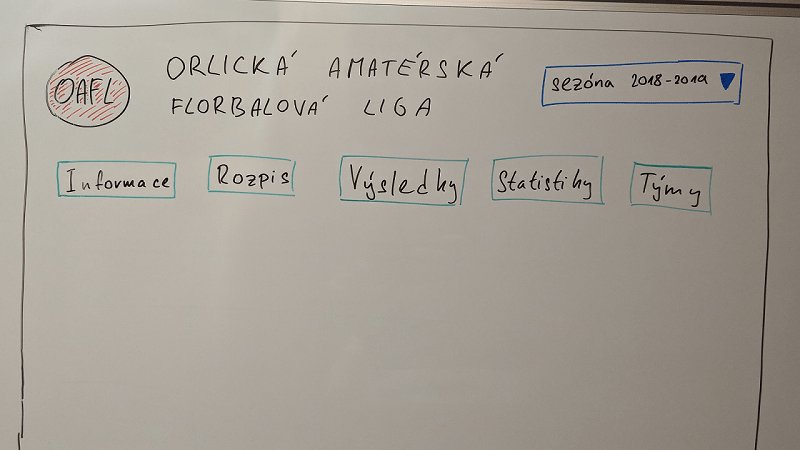
\includegraphics[width=.98\textwidth]{images/draft-01.png}
        \captionof{figure}{Návrh GUI}
    \end{minipage}%
    \begin{minipage}{.5\textwidth}
        \centering
        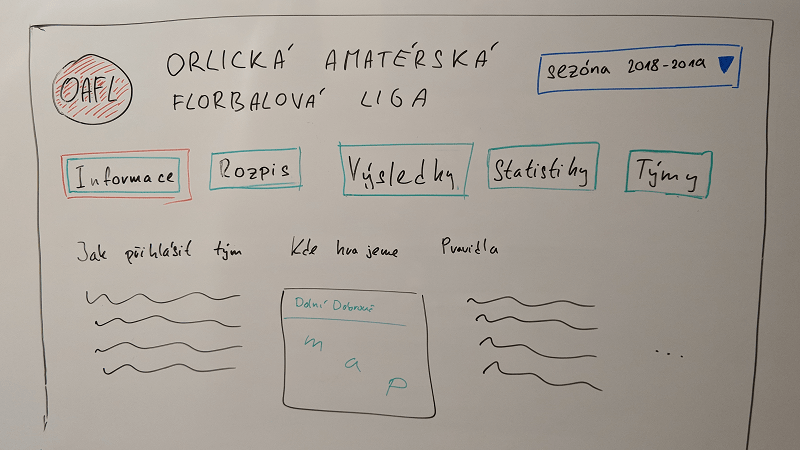
\includegraphics[width=.98\textwidth]{images/draft-02.png}
        \captionof{figure}{Návrh GUI}
    \end{minipage}
\end{figure}

\begin{figure}[H]
\centering
    \begin{minipage}{.5\textwidth}
        \centering
        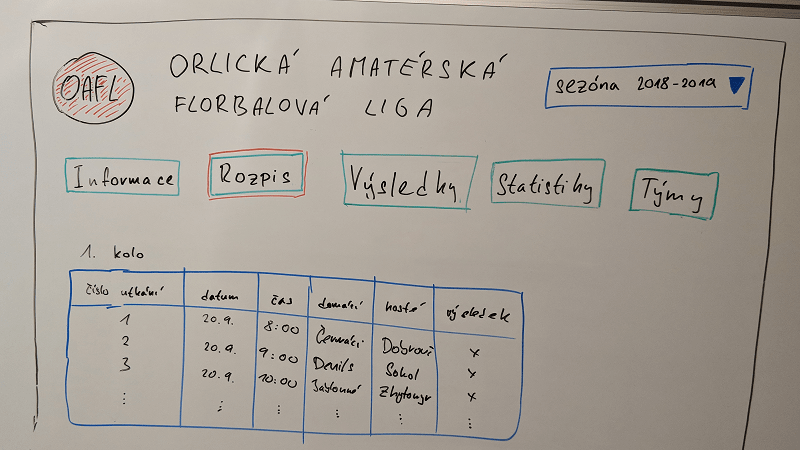
\includegraphics[width=.98\textwidth]{images/draft-03.png}
        \captionof{figure}{Návrh GUI}
    \end{minipage}%
    \begin{minipage}{.5\textwidth}
        \centering
        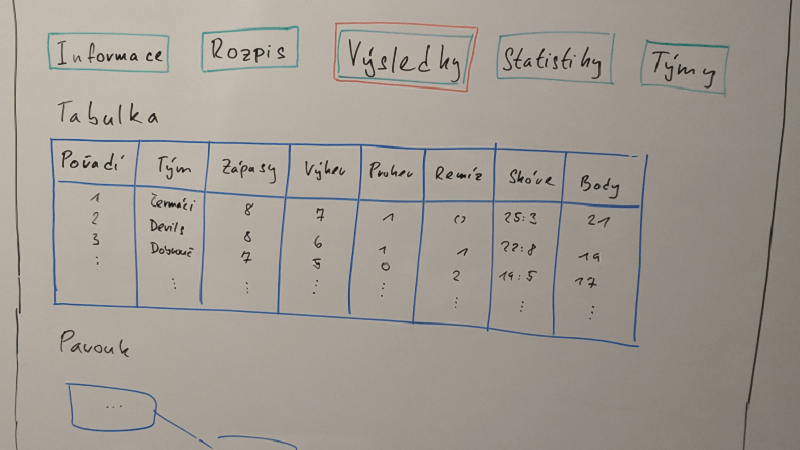
\includegraphics[width=.98\textwidth]{images/draft-04.png}
        \captionof{figure}{Návrh GUI}
    \end{minipage}
\end{figure}

\begin{figure}[H]
\centering
    \begin{minipage}{.5\textwidth}
        \centering
        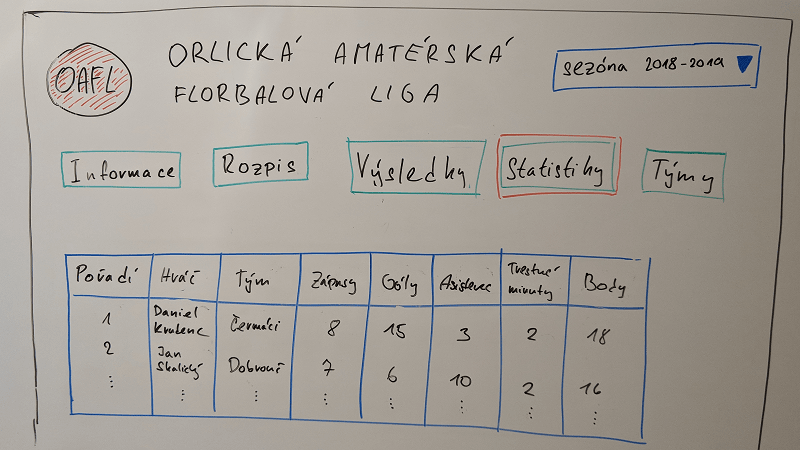
\includegraphics[width=.98\textwidth]{images/draft-05.png}
        \captionof{figure}{Návrh GUI}
    \end{minipage}%
    \begin{minipage}{.5\textwidth}
        \centering
        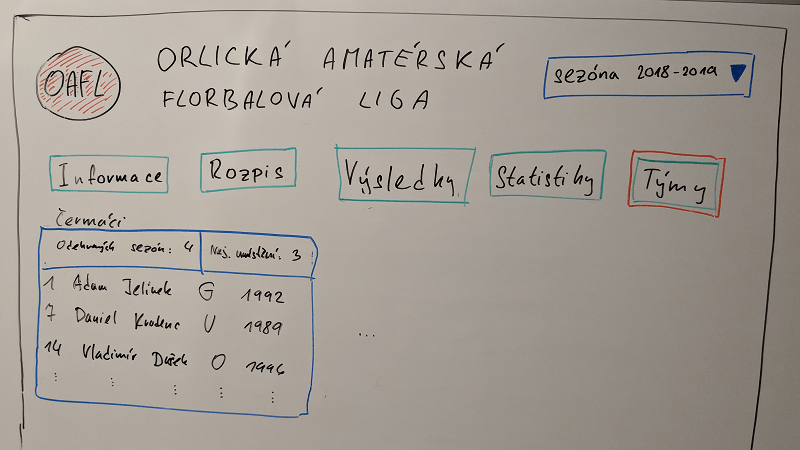
\includegraphics[width=.98\textwidth]{images/draft-06.png}
        \captionof{figure}{Návrh GUI}
    \end{minipage}
\end{figure}

%%%%%%%%%%%%%%%%%%%%%%%%%%%%%%%%%%%%%%%%%%%%%%%%%%%%%%%%%%%%%%%%%%%%%

\newpage

\section{Testování prototypu GUI}

\subsection{Individuální návrh testování}

Snažil jsem se o jednoduché a přehledné rozhraní, bez zbytečností a rušivých elementů. Také jsem měl v úmyslu co nejvíce zachovat dosavadní systém řazení informací. Tedy tabulku pro výsledky, pro rozpisy zápasů, pro kanadské bodování a podobně. Grafické uživatelské rozhraní webu jsem promyslel, navrhl a načrtnul.

\subsection{Realizace testů}

Výsledný náčrt jsem představoval jedincům z cílové skupiny uživatelů, se kterými jsem se osobně sešel. Vybral jsem zástupce z organizátorů, hráčů i potenciálních fanoušků.

\subsection{Výsledky a závěry}

Běhěm diskuze s vybranými respondenty jsem přišel na nové informace a získal pohled od potenciálních uživatelů. Hlavně jsme se bavili o rozložení položek menu a co pod nimi nalezneme. Prvotní návrh působil najednoznačně a vyvolával otázky typu co je kde.
\medskip

Položka Rozpis by mohla být nahrazena více vystihujícím názvem Program. Případně při najetí myši, by se zobrazil popis, který bude upřesňovat, že se jedná o rozpis zápasů.
\medskip

Stránka Výsledky by podle původního návrhu obsahovala výsledky všech zápasů, průběžnou tabulku a v případě play-off i pavouka. To je značně matoucí, proto každému tomuto prvku přidáme v menu samostatnou položku.
\medskip

Stránka Informace bude přejmenována na O nás a bude zároveň domovskou stránkou.
\medskip

Jako inspirace rozložení informací můžou posloužit stránky \path{www.ceskyflorbal.cz}. Ty slouží pro zaznamenávání informací o české extralize ve florbalu. Případně \path{www.livesport.cz}, kde jsou výsledky z mnoha sportů.
\medskip

S případnými drobnými úpravami zachováme i původní logo OAFL (Obrázek \ref{fig:logo}). Hráči jsou na něj zvyklí a působí nostalgickým dojmem. Design webu mu bude přizpůsoben.
\medskip

Upravené menu je vidět na Obrázku \ref{fig:menu}. Při najetí myši na každou položku se zobrazí upřesňující popis.

\begin{figure}[H]
\centering
    \begin{minipage}{.5\textwidth}
        \centering
        
\includegraphics[width=.60\textwidth]{images/logo.jpg}
        \captionof{figure}{Logo}
        \label{fig:logo}
    \end{minipage}%
    \begin{minipage}{.5\textwidth}
        \centering
        
\includegraphics[width=.99\textwidth]{images/menu.png}
        \captionof{figure}{Menu} \label{fig:menu}
    \end{minipage}
\end{figure}

%%%%%%%%%%%%%%%%%%%%%%%%%%%%%%%%%%%%%%%%%%%%%%%%%%%%%%%%%%%%%%%%%%%%%

\newpage

\section{Implementace}

Obsahem této kapitoly jsou záležitosti ohledně volby technologií pro tvorbu webového back-endu a front-endu. Kapitola zároveň obsahuje snímky s finálním uživatelským rozhraním.

\subsection{Výběr technologií}

Pro tvorbu back-endu jsem se rozhodl využít Python web framework Django s databází PostgreSQL. Jedná se o vysokoúrovňový framework, který například programátora ušetří psaní SQL dotazů, dotaz se specifikuje přímo v Pythonu. Zároveň poskytuje HTML šablonovací systém pro tvoření dynamické tvoření HTML dokumentů. Pro tvorbu front-endu jsem se rozhodl využít CSS framework Bootstrap3, který poskytuje velké množství již implementovaných tříd stylů.

\subsection{Back-end}

Za klíčovou funkci back-endu považuji administrátorské rozhraní Django admin, které jsem upravil pro potřeby OAFL. Organizátoři soutěže budou moci pohodlně vypisovat nové zápasy, vyplňovat výsledky odehraných zápasů, střelce gólů a podobně. Na následujícím obrázku je zobrazeno upravování zápasu.

\begin{figure}[H]
    \centering
    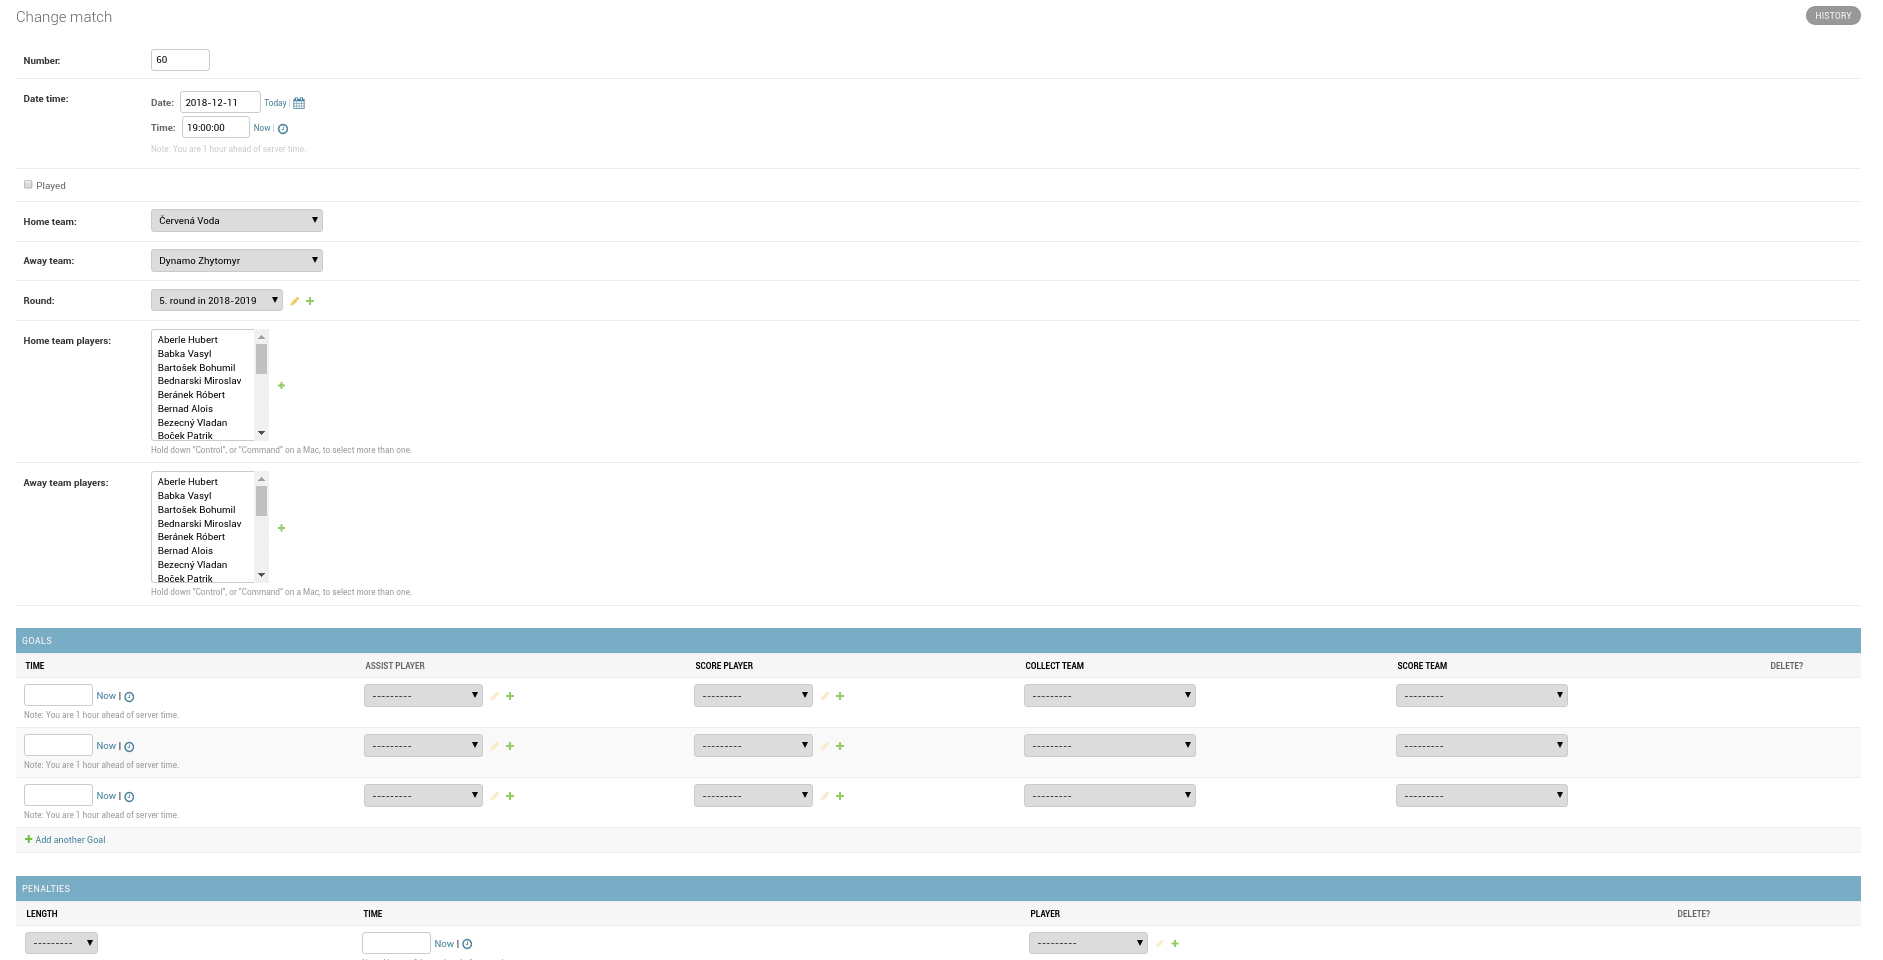
\includegraphics[width=.99\textwidth]{images/admin.png}\hfill
    \caption{Administrátorské rozhraní pro úpravu zápasu}
\end{figure}

\subsection{Front-end}

\subsubsection{Výsledné rozložení prvků}

Grafické rozhraní by se dalo rozdělit na tři části. Hlavičku, kde se nachází logo a název soutěže. Navigační lištu s jednotlivou nabídkou stránek a comboboxem pro změnu sezóny. A poslední obsah jednotlivých stránek.

\begin{figure}[H]
    \centering
    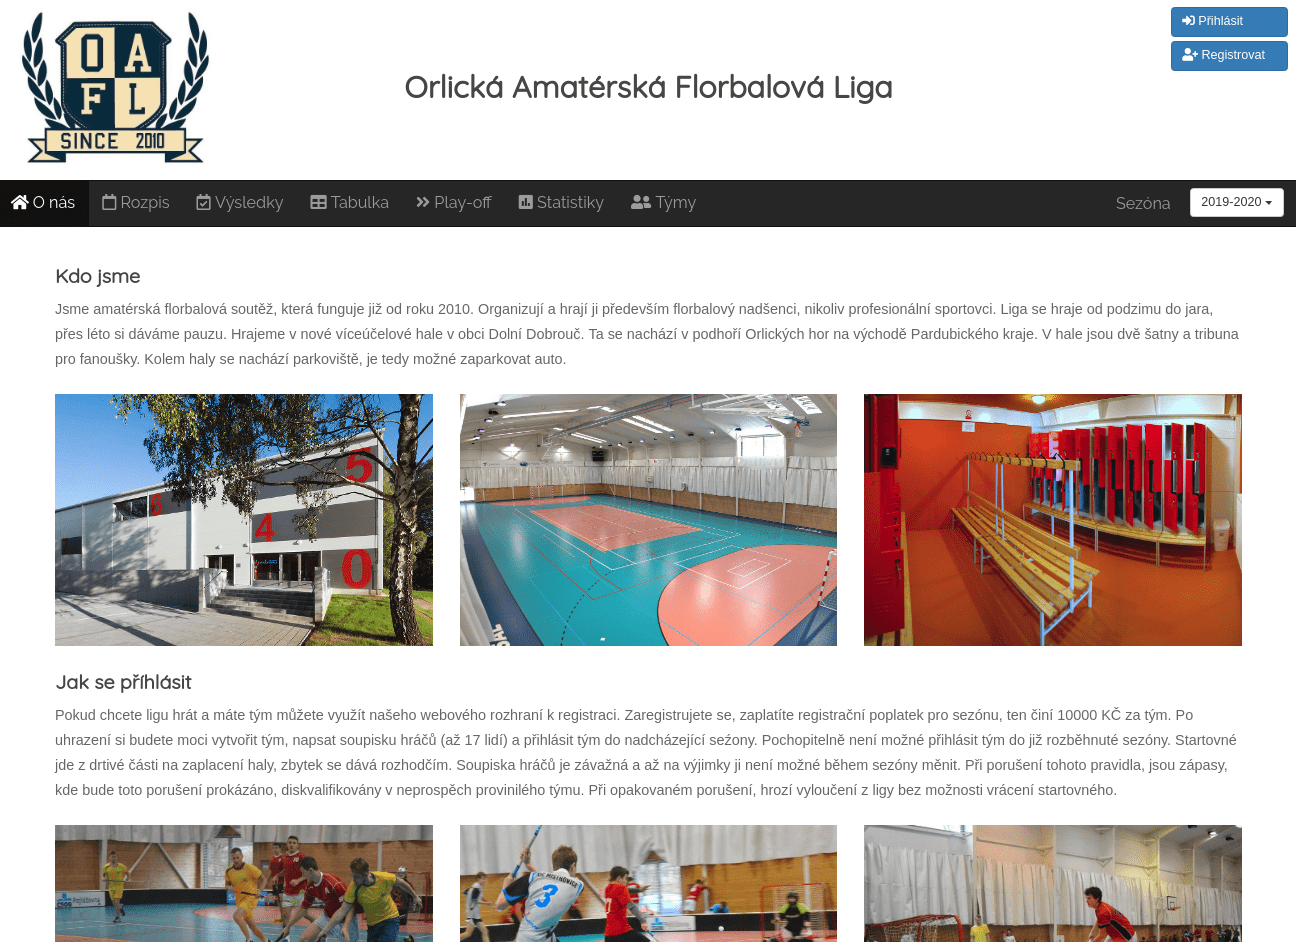
\includegraphics[width=.8\textwidth]{images/home.png}\hfill
    % \caption{Rozložení stránky}
\end{figure}


\subsubsection{Rozpis}

Na stránce Rozpis můžeme najít kdy se hrají jednotlivé zápasy. Každé kolo na jedné stráně a barevně odlišené odehrané/neodehrané zápasy.

\begin{figure}[H]
    \centering
    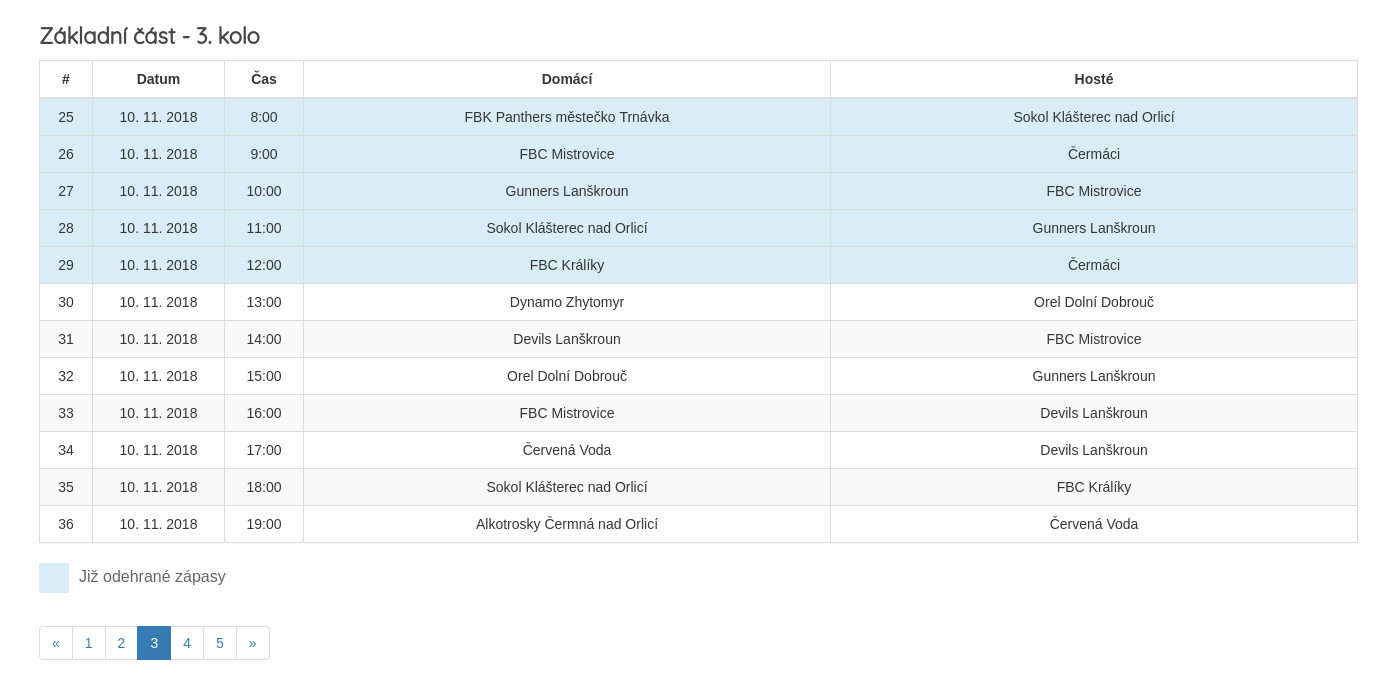
\includegraphics[width=.8\textwidth]{images/rozpis.png}\hfill
    % \caption{Stránka Rozpis}
\end{figure}



\subsubsection{Výsledky}

Stránka Výsledků pak obsahuje pouze odehrané zápasy. Po kliknutí na zápas se zobrazí detail zápasu - v jaké minutě padnul gól, kdo ho vštřelil, případně kdy a komu byl udělen trest. Každé kolo je opět na samostatné stráně.

\begin{figure}[H]
    \centering
    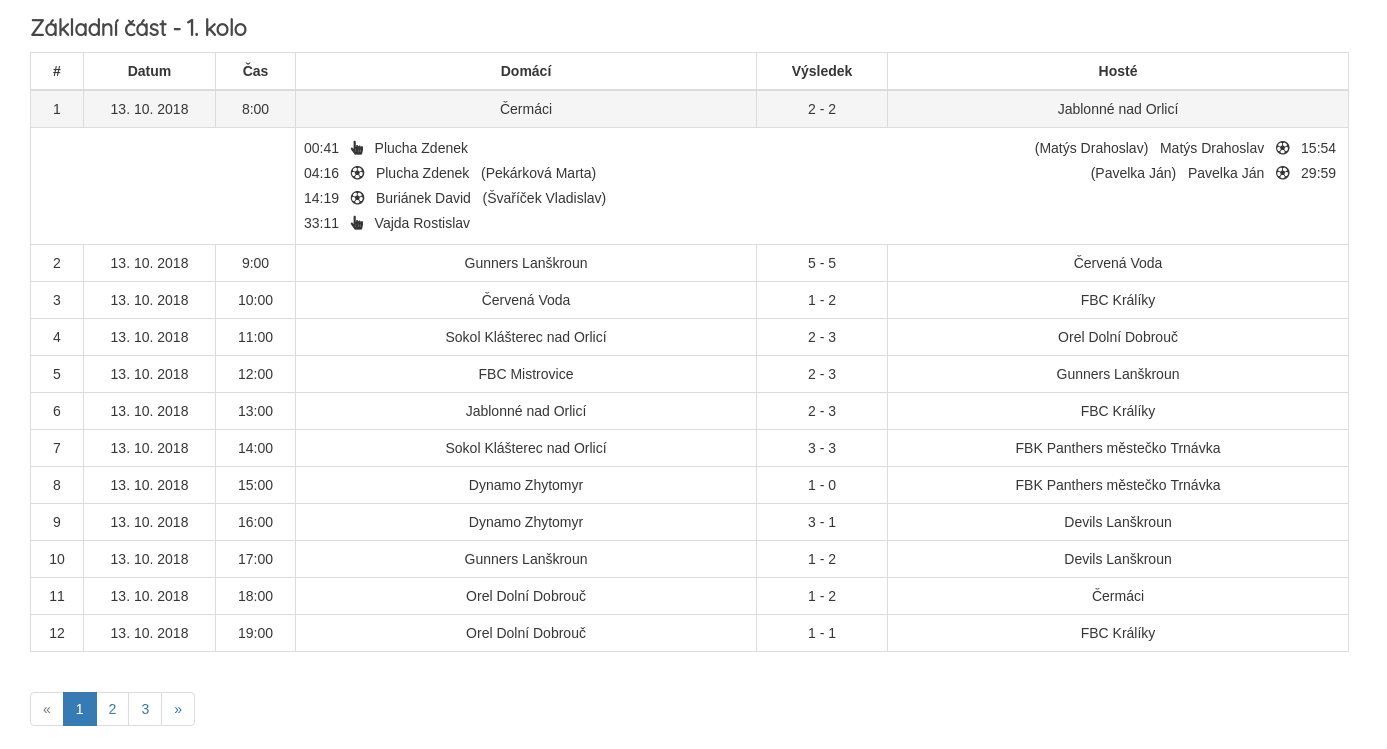
\includegraphics[width=.8\textwidth]{images/vysledky.png}\hfill
    % \caption{Stránka Výsledky}
\end{figure}



\subsubsection{Tabulka}

Stránka Tabulka obsahuje průběžné či konečné pořadí týmů v základní části. Barevně jsou zvýrazněny postupová místa do vyřazovací části.

\begin{figure}[H]
    \centering
    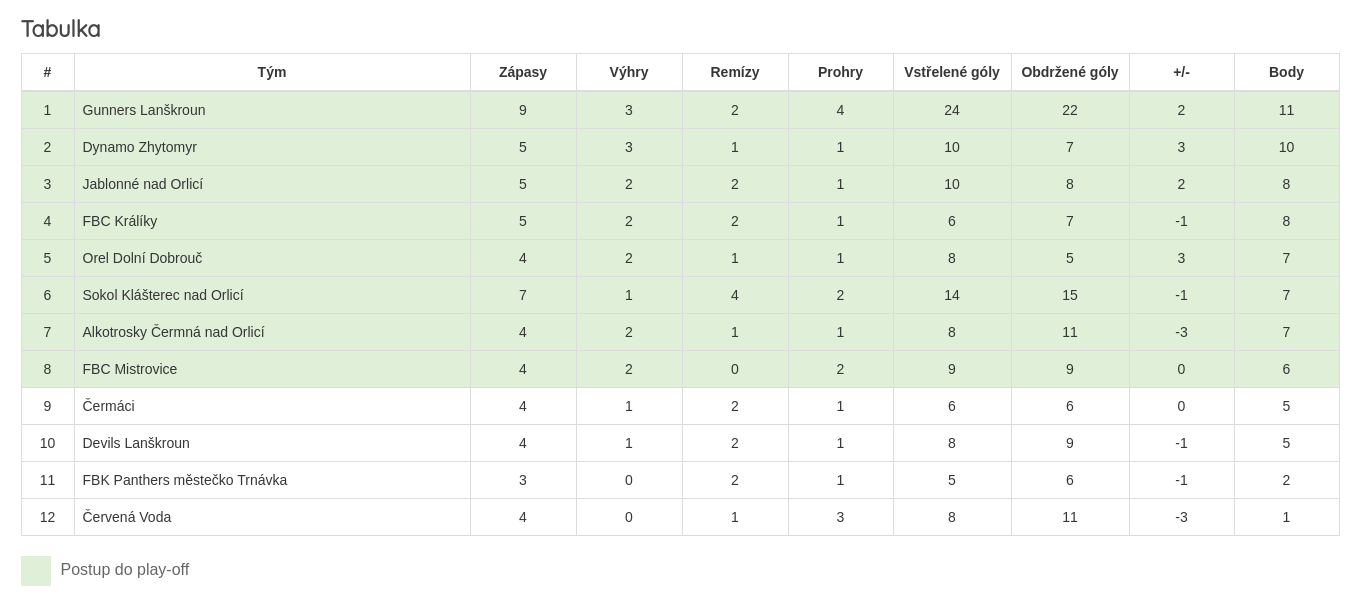
\includegraphics[width=.8\textwidth]{images/tabulka.png}\hfill
    % \caption{Stránka Tabulka}
\end{figure}



\subsubsection{Play-off}

Na stránce play-off je zobrazeno rozdělení pavouka pro vyřazovací část sezóny. Uživatel tak může vidět, na jaké soupeřě může jeho tým v dalších kolech narazit.

\begin{figure}[H]
    \centering
    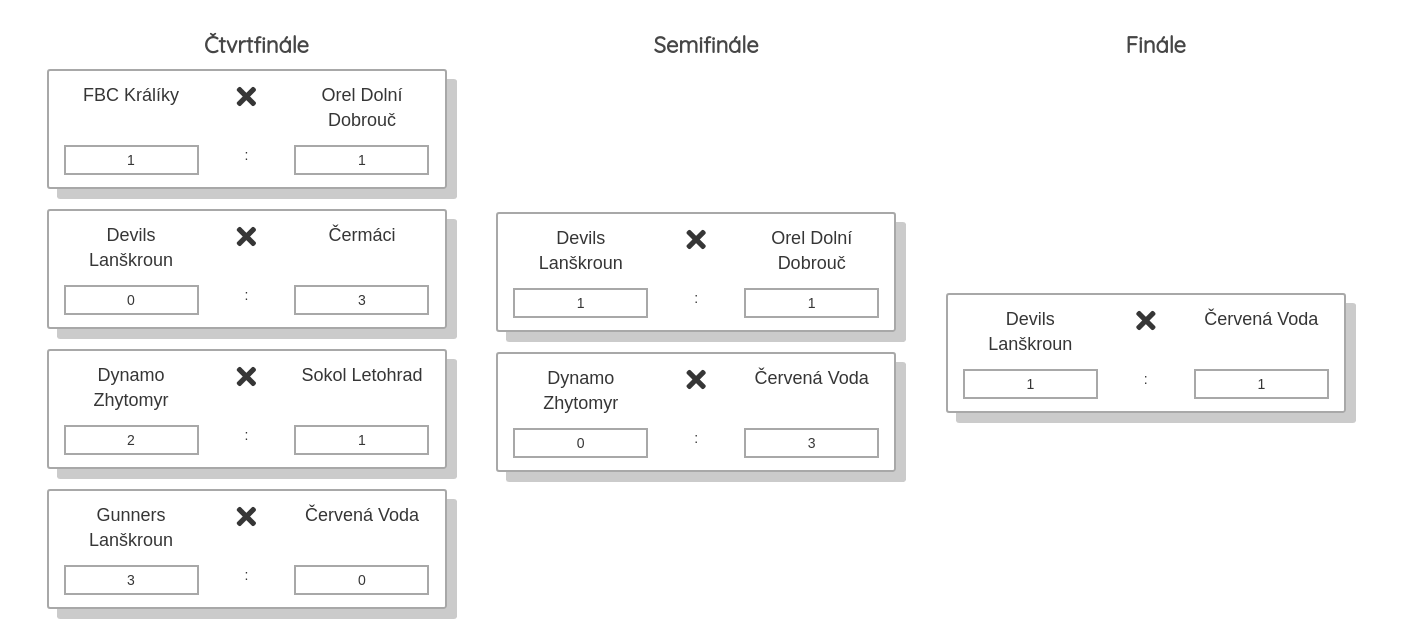
\includegraphics[width=.8\textwidth]{images/play-off.png}\hfill
    % \caption{Stránka Play-off}
\end{figure}



\subsubsection{Statistiky}

Na stránce Statistik pak můžeme najít všechny hráče registrované v dané sezóně a zjistit jak se jim daří, případně jak moc se proviňují proti pravidlům.

\begin{figure}[H]
    \centering
    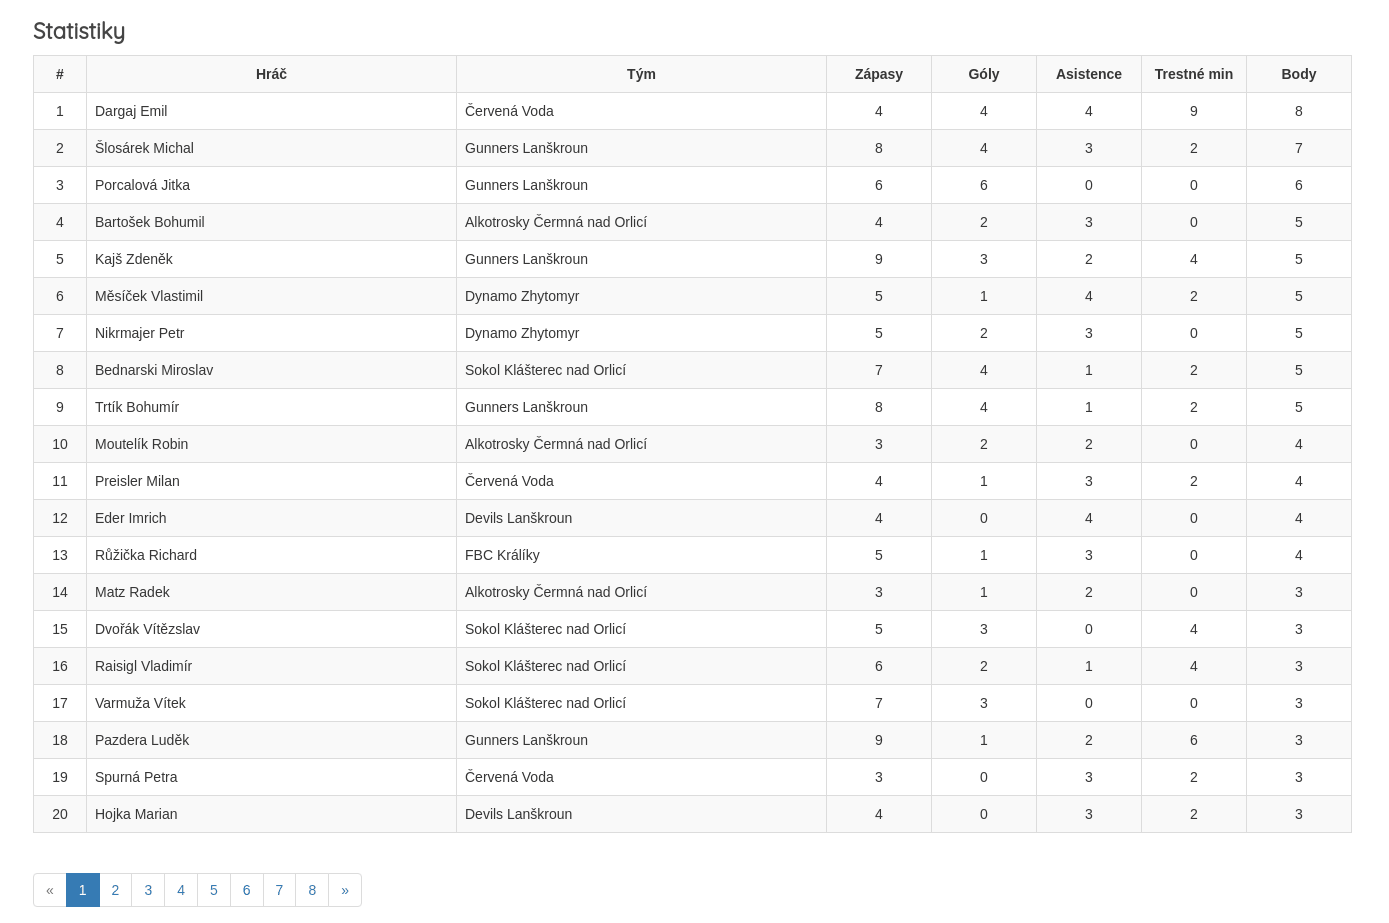
\includegraphics[width=.8\textwidth]{images/statistiky.png}\hfill
    % \caption{Stránka Statistiky}
\end{figure}



\subsubsection{Týmy}

Poslední stránka Týmy pak zobrazuje týmy které danou seźonu hrají. Zároveň můžeme najít nějaké další informace o týmu, jako například kolik sezón již odehrál a jak se nejlépe umístil. Také je možnost si po rozkliknutí týmu zobrazit soupisku hráčů.

\begin{figure}[H]
    \centering
    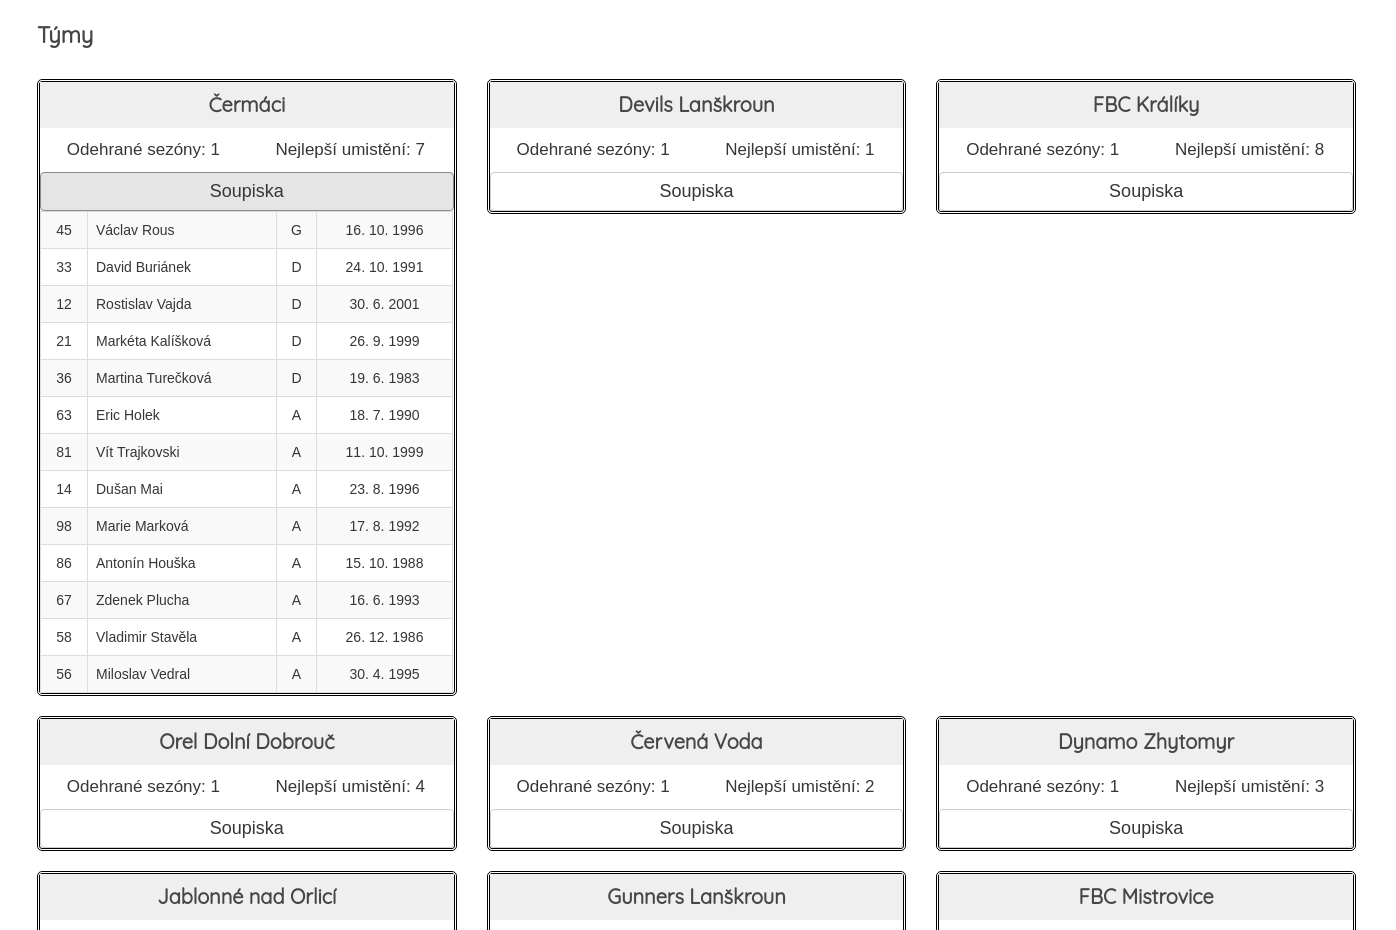
\includegraphics[width=.8\textwidth]{images/tymy.png}\hfill
    % \caption{Stránka Týmů}
\end{figure}

%%%%%%%%%%%%%%%%%%%%%%%%%%%%%%%%%%%%%%%%%%%%%%%%%%%%%%%%%%%%%%%%%%%%%

\newpage

\section{Závěr}

Na základě protypu a zpětné vazby na něho jsem upravil rozložení stránek a jejich obsah. Věřím, že to pomůže uživatelům se na webu rychle zorientovat a budou vědět co kde hledat.

Vytyčené cíle se až na výjimky podařilo splnit. Například nejsou dostupné doplňující statistiky za celou seźonu, jako kolik bylo celkem vstřeleno gólů, průměrný počet gólů na zápas, kolik bylo uděleno trestů a podobně. Zároveň není možné data v tabulkách řadit uživatelem. Uživatel by například mohl kliknutím na sloupec seřadit řádky tabulky. Mohl by se tak dostat k dalším informacím, jako například tým který nejlépe brání, hráč který nejvíce nahrává, nejtrestanější hráč a podobně.

%%%%%%%%%%%%%%%%%%%%%%%%%%%%%%%%%%%%%%%%%%%%%%%%%%%%%%%%%%%%%%%%%%%%%

\end{document}
